% include the figures path relative to the master file
\graphicspath{ {./content/method/figures/} }

\section{Segmentation methodology description} 

Optimization methodologies offer a standardized manner to approach segmentation by minimizing an application-driven cost function~\cite{cremers2007review}.
\Cref{fig:method} illustrates a generic representation of the segmentation strategy here adopted to delineate breast tissues or lesions in \ac{us} images. 
The overall segmentation can be seen as a three-step strategy: 
(1) a mapping or encoding of the image into a discrete set of elements $\mathcal{S}$, 
(2) the optimization stage which is formulated as \emph{metric labelling} problem, 
and (3) re-mapping the labels obtained from the previous stage to produce the final delineation. 

\begin{figure}[htpb]
  \centering
  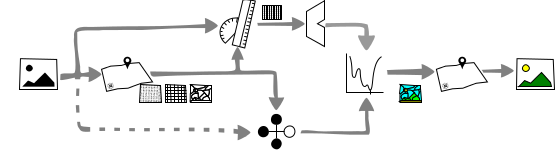
\includegraphics[width=0.9\linewidth]{method}
  \caption{Conceptual block representation of the segmentation methodology}
  \label{fig:method}
\end{figure}

In order to formulate the segmentation like a metric labelling problem, the image is conceived as a discrete set of elements $\mathcal{S}$ that need to be labelled using a label $l$ from the labelling set $\mathcal{L}$ 
(i.e.\, $l \in \{\text{lesion}, \overline{\text{lesion}}\}$ 
or $l \in \{\text{lungs}, \text{fat},\,\cdots\,, \text{lesion}\}$).
Let $\mathcal{W}$ be all the possible labelling configurations of the set $\mathcal{S}$ given $\mathcal{L}$; and, let $U(\cdot)$ be a cost function encoding how good is a labelling configuration $\omega \in \mathcal{W}$ based on the appearance of the elements in $\mathcal{S}$, their inner relation and some desig constraints.
Then, the desired segmentation $\hat{\omega}$ corresponds to the labelling configuration that minimize this cost function, as described in \cref{eq:costMin}.

\begin{equation}
\hat{\omega} = \arg \min_{\substack{\omega}} \,U(\omega)
\label{eq:costMin}
\end{equation}

The nature of $U(\cdot)$ and $\mathcal{W}$ dictates which minimization strategies should be applied to find $\hat{\omega}$ sine not every strategy is suitable or desirable.

\Cref{eq:labelingeq} determines this cost function as the combination of two independent costs that need to be simultaneously minimized as a whole.
The left hand side of the expression integrates the so called \emph{data} term, while the right hand side integrates the \emph{pairwise} term, which is also referred as the \emph{smoothing} term.
Both terms are shaped by $\mathcal{S}$ and evaluated in $\mathcal{W}$.

\begin{equation}
  U(\omega) = \sum_{s\in s} D_s(\omega_s) + \sum_{s}\sum_{r \in \mathcal{N}_{s}} V_{s,r}(\omega_s,\omega_r)
  \label{eq:labelingeq}
\end{equation}

\Cref{fig:methodterms} illustrates the terms and elements relating the framework's outline, presented in \cref{fig:method}, with its formulation in \cref{eq:labelingeq}.
The problem of delineating the tissues present in \ac{bus} image has been used here for this illustrative purposes. 

\begin{figure}
    \centering
    \begin{subfigure}[b]{0.19\textwidth}
        \centering
        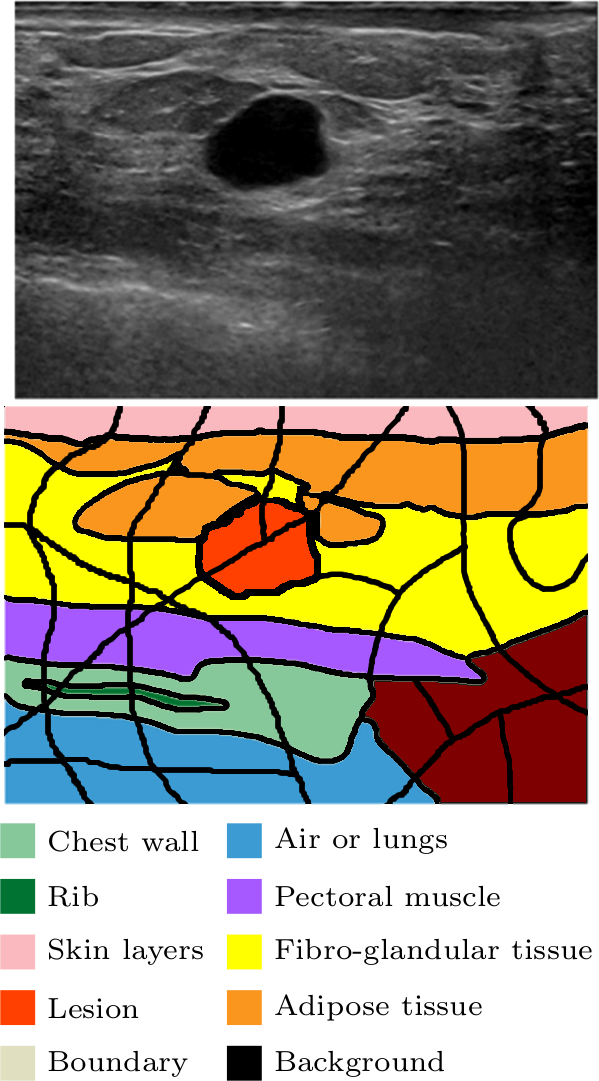
\includegraphics[width=\textwidth]{problem}
        \caption{{\small Problem definition}}    
        \label{fig:methodTerms:problem}
    \end{subfigure}
    \hfill
    \begin{subfigure}[b]{0.39\textwidth}  
        \centering 
        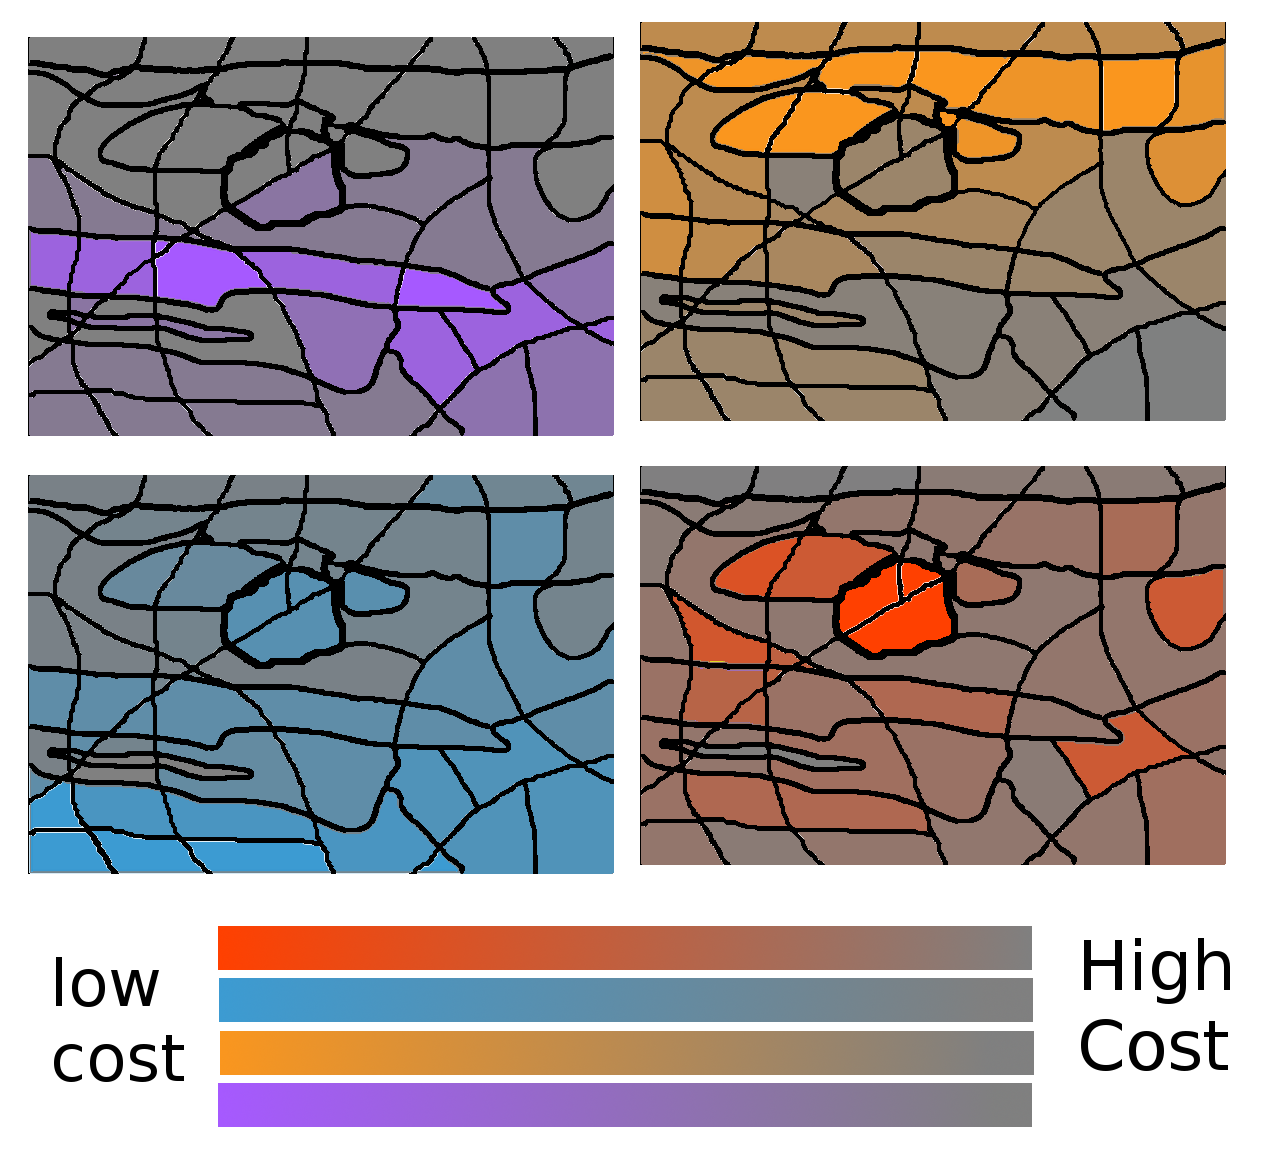
\includegraphics[width=\textwidth]{data}
        \caption[]%
        {{\small Data term}}    
        \label{fig:methodTerms:data}
    \end{subfigure}
    \hfill
    \begin{subfigure}[b]{0.39\textwidth}   
        \centering 
        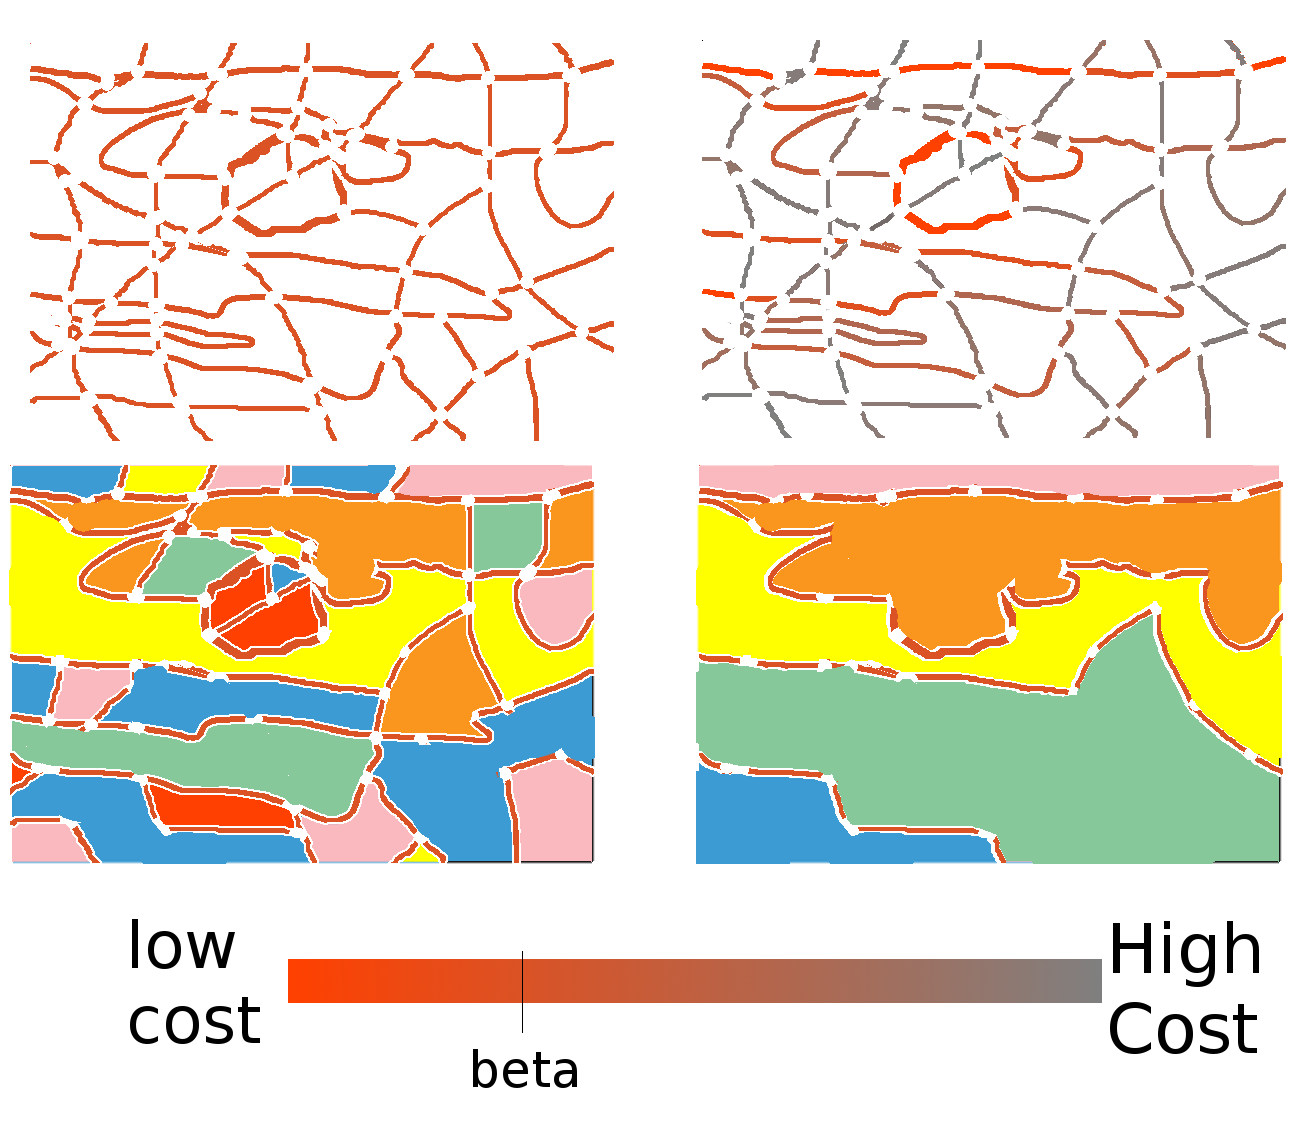
\includegraphics[width=\textwidth]{smooth} \caption[]%
        {{\small Pairwise term \emph{for this term the labels should be patterns and the cost be the only colour}}}    
        \label{fig:methodTerms:boundary}
    \end{subfigure}
    \caption {\small Methodology terms interpretation} 
    \label{fig:methodterms}
\end{figure}

In general, $\mathcal{S}$ can be any discrete set representing the image (i.e.\, pixels, overlapping or non overlapping windows, etc.). 
For this work $\mathcal{S}$ is chosen to be a super-pixels representation of the image~\cite{achanta2012slic}, though. 
% Good % The super-pixels can be seen as the output of a over-segmentation process or as a set of pixel collections that are contiguous and coherent with respect to some metric. Either way super-pixels are no overlapped irregular groups of similar connected pixels~\cite{achanta2012slic}.
\Cref{fig:methodTerms:problem} shows a \ac{bus} image example and a its associated super-pixels representation $\mathcal{S}$ coloured according to the image's \ac{gt}.

Bear in mind that given an unseen \ac{bus} image, the ultimate goal is to represent the image as a set of super-pixels and infer the appropriated labelling for each of them.
To do so using the strategy here proposed, it requires to define: a data term, a pairwise term, and a proper minimization methodology.

\subsection{Data term} \label{sec:method:dataTerm}

Given a label configuration $\omega \in \mathcal{W}$, the data term penalizes the 
labelling of a particular image element or site ($\omega_s = l$) based on the data associated to $s$. 
In this manner $D_s(\omega_s=l_\cmark) << D_s(\omega_s=l_\xmark)$. 
To perceive the effect or behaviour of this data term, \cref{fig:methodTerms:data} shows some labelling configurations $\omega'$ where all the sites share the same label, $\omega' \in \{ \omega_s=l,~\forall s\in\mathcal{S}\}$

Designing $D(\cdot)$ that accomplish the desired behaviour by defining an obscure heuristic, is rather complicated task to achieve out of the box. 
Therefore, an easier and cleaner approach is to take advantage of \ac{ml} techniques to design this data cost in a systematic manner based on a training stage. 
The idea is to generate image or data model for each class from training samples, and let $D(\cdot)$ be a distance or goodness measure reflecting the likelihood for $s$ to to belong to class $l$.
Defining the data term in this manner allows for great flexibility while offering a systematic approach towards its design.  
$D(\cdot)$ is fully customizable through the features, through the construction of the model where several classifiers and training techniques can be applied; or through definition of the relation between the testing sample and the data models. 

This type of data term is incorporated to our framework as represented at the upper side of the diagram in \cref{fig:method}.
Each site $s$ is treated as a sample and the features to describe it are extracted from the original image. 
For the work here reported, a \ac{svm} classifier is used to determine the data model during the training stage.
During testing stage $D_s(\omega_s=l)$ corresponds to the distance between the testing sample and the model associated to $l$ as the \ac{svm} classification reward. 

%Further discussion regarding the feature choices can be found in \cref{sec:featuers}, whereas other designing choices regarding \ac{ml} are out of the scope for this work.

The final manuscript has a section dedicated to describe and analyse the features designed for \ac{bus} images based in \cref{fig:lesions}. Other analysis regarding the \ac{ml} stage are out of the study here presented.

\subsection{Pairwise or smoothing term} \label{sec:method:mrfTerm}
 
The pairwise term represents the cost of the assignation $\omega_s$ taking into account the labels of its neighbour sites, $\omega_r$, $r \in \mathcal{N}_{s}$. 
This term models a \ac{mrf} or a \ac{crf}.
The typical form of this term, given in \cref{eq:smoothing}, is called homogenization which acts as a regularization factor favouring configurations that have coherent labelling.

\begin{equation}
V_{s,r}(\omega_s,\omega_r) = 
\begin{cases}
    \beta, & \text{if } \omega_s \ne \omega_r\\
    0,              & \text{otherwise}
\end{cases}
\label{eq:smoothing}
\end{equation}

\Cref{fig:methodTerms:boundary} offers a visual interpretation of this cost.
If the resulting segmentation associated to the current labelling configuration $\omega$ has a boundary segment, this boundary brings a penalization $\beta$ to the total cost $U(\omega)$.
In this manner the regularization term can be seen as a post-processing or denoising stage since some sites will flip their labelling if the cost of producing and edge is larger than the cost of adopting the neighbour's label. 

More sophisticated smoothing terms where boundaries have different penalization based not only on site relations in $\mathcal{S}$ but also based on image information would (see \cref{fig:methodTerms:boundary}) be found in the final version of the manuscript.% in \cref{sec:smoothing}.

% Review %contribute have different or variable costs (see \cref{fig:methodTerms:boundary}) are also possible by taking into account not only relations in $\mathcal{S}$ of but also image information (see \cref{fig:method}). 
%Further details can be found in \cref{sec:smoothing}.

\subsection{Searching the best labelling configuration}
Once defined $U(\omega)$ so that the cost for a particular labelling configuration $\omega$ can be computed, the problem of finding $\hat{\omega}$ corresponding to the global minimum of the space $\mathcal{W}$ of all possible labelling configurations needs to be faced. 

This problem falls into the category of \textbf{NP-hard} problems. 
% Good % The dimension of the solution space can be expressed as $||\mathcal{W}|| = ||\mathcal{L}||^{||\mathcal{S}||}$. 
% Good % This means that in order to perform an exhaustive search for a toy example of $20$ sites and two possible labels, the cost function needs to be calculated way more than a million times. 
More over, due to limitations in building $U(\cdot)$ such as noise, training policies, etc. there are no guarantees that the global minimum $\hat{\omega}$ corresponds to the true labelling.

Nevertheless, there is a large body of literature proposing methodologies to find suboptimal solutions to the problem trading-off between time of convergence and accuracy of the solution reached.
Szeliski et al.~\cite{szeliski2008comparative} conducted an exhaustive review in terms of solution quality and runtime of the most common energy minimization algorithms used in \ac{cv}, such as \ac{icm}, \ac{sa} or \ac{gc}.

The minimization strategy used for this work is \ac{gc}. 
This technique was initially introduced to solve \ac{cv} applications by Boykov et al.~\cite{boykov2001fast}.
Soon after its introduction, it become the minimization technique of choice for \ac{cv} problems.
Since, when \ac{gc} is applicable, it allows to rapidly find a strong local minima guaranteeing that no other minimum with with lower energy can be found~\cite{delong2012fast}. 
\ac{gc} is applicable if, and only if, the pairwise term favours coherent labelling configurations and penalizes labelling configurations where neighbours labels differs. 
Such is our case, given \cref{eq:smoothing}.

% Good % \subsection{Similitude with other optimization techniques}
% Good % \todo{needs reworking}
% Good % It is worth to mention here, that this pairwise term links this segmentation strategy to the family of segmentation methodologies based on optimization using \ac{acm}, such as levelsets.
% Good % On its basic form, the family of \ac{acm} segmentation defines some forces to be applied to an initial contour and this contour evolves by minimizing its length while constrained by the forces properly designed for the task in hand.

%%% Local Variables: 
%%% mode: latex
%%% TeX-master: "../../master.tex"
